\section{Сбор и анализ требований}
\subsection{Этап сбора требований}

\label{req:sect_1}

Подэтапы сбора требований включают в себя:

\begin{itemize}[wide]
    \item Анкетирование целевой аудитории;
    \item Изучение рынка на предемет конкурентов;
    \item Мозговой штурм.
\end{itemize}

\subsubsection{Анкетирование целевой аудитории}

В рамках сбора требований к программному продукту было проведено анкетирование целевой аудитории проекта. В состав анкеты вошли следующие вопросы:

\begin{enumerate}
    \item "<Кто вы в IT?">;
    \item "<Часто ли вы имеете дело с файлом docker-compose.yaml?">;
    \item "<Используете ли вы специальные средства для редактирования docker-compose.yaml?">;
    \item "<Хотели бы вы иметь под рукой графический интерфейс со множеством возможностей для редактирования docker-compose.yaml?">;
    \item "<Пожалуйста, опишите желаемые возможности подобного инструмента.">.
\end{enumerate}

Диаграмма ответов на первый вопрос привидён на рисунке \ref{req:first_q}.

\begin{figure}[H]
        \center{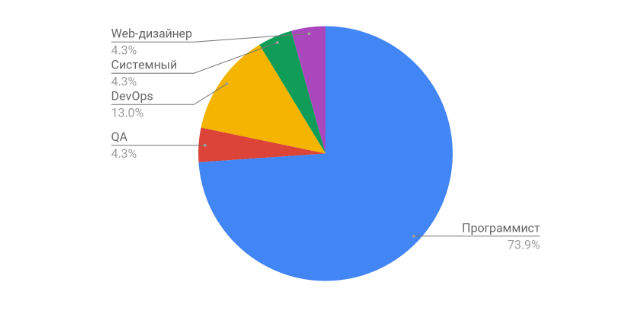
\includegraphics[scale=0.7]{first_q.png}}
        \caption{Ответы на первый вопрос анкеты}
        \label{req:first_q}
\end{figure}

Ответы на первый вопрос поможет уточнить уточнить состав целевой аудитории по направлениям в IT.

Исходя из результатов, отображённых на рисунке \ref{req:first_q} можно сделать следующие выводы:
\begin{itemize}
    \item не потребуется поддержка старых браузеров, так как программисты технически заточены и шанс, что кто-то из них будет использовать Internet Explorer ниже 11 версии низок;
    \item цветовая палитра рабочей области должна быть в тёмных тонах, так как большинство программистов используют в IDE и текстовых редакторов тёмную тему оформления.
\end{itemize}

Диаграмма результатов ответа на второй вопрос привидена на рисунке \ref{req:second_q}.

\begin{figure}[H]
    \center{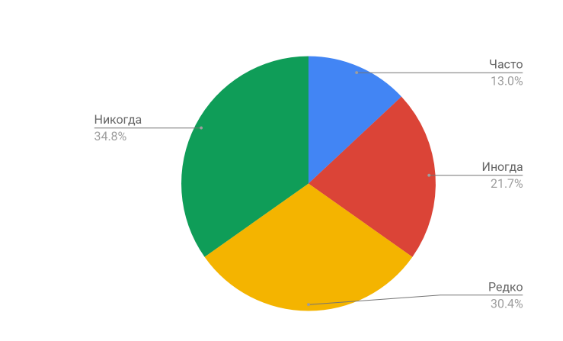
\includegraphics[scale=0.7]{second_q.png}}
    \caption{Ответы на второй вопрос анкеты}
    \label{req:second_q}
\end{figure}

Ответы помогут нам понять, как часто будет пригождаться тем или иным пользователям наш продукт. Делая вывод, можно понять, что
требуется сделать акцент на том, что значительная часть пользователей сервиса будут использовать его не единожды. Это значит, что нужно дать пользователю возможность получать доступ к ранее созданным файлам конфигураций в рамках сервиса. За это должна взиматься плата в виде ежемесячной подписки.

Ответы на третий вопрос позволяют узнать ранее незамечанных конкурентов при разработке идеи проекта. Абсолютно все участники опроса ответили на него отрицательно.

Диаграмма ответов опрашиваемых на четвёртый вопрос привидена на рисунке \ref{req:fourth_q}.

\begin{figure}[H]
    \center{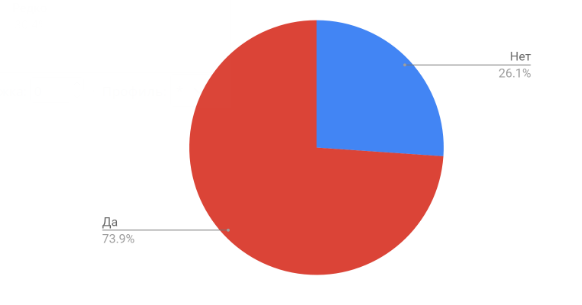
\includegraphics[scale=0.7]{fourth_q.png}}
    \caption{Ответы на четвёртый вопрос анкеты}
    \label{req:fourth_q}
\end{figure}

Ответы на четвёртый вопрос являются главными для проекта, иными словами нужен ли рынку разрабатываемый программный продукт.

Ответов на четвёртый вопрос, к сожалению не поступило.

\subsubsection{Изучение рынка}

В процессе поиска конкурирующего программного обеспечения не было обнаружено серьёзных соперников в данной области. Исключение составляют лишь инструменты, являющиеся обособленными частями рассматриваемого проекта, как то:

\begin{itemize}[wide]
    \item Инструменты для проверки синтаксиса;
    \item Текстовые редакторы;
    \item Различные документации.
\end{itemize}

Также об отсутствии конкурентов на рынке свидетельствуют и результаты анкетирование, приведённые в пункте 1.1.1.

\subsubsection{Мозговой штурм}

По результатам данного этапа сбора требований были выдвинуты следующие идеи:

\begin{itemize}
    \item должно сущестовать две роли пользователей: посетитель и клиент;
    \item в качестве встроенного текстового редактора нужно использовать Monaco Editor - редактор с открытым исходным кодом и большим количеством возможностей в настройке, который можно встраивать на сайт;
    \item приложение не будет активно использоваться на мобильных устройствах, а из этого следует:
    \begin{itemize}
        \item достаточно поддержки десктопных браузеров;
        \item адаптивность страниц под мобильные устройства не требуется.
    \end{itemize}
    \item необходимо наличие сервера, который бы предоставлял данные с базы данных;
    \item необходимо наличие авторизационного сервера, предоставляющего функционал связанные с аутенфикацией и авторизацией.
\end{itemize}

\subsection{Этап анализа и формирования требований}

\label{req:sect_2}

Исходя из темы дипломной работы, необходимо обозначить требования к серверной части проекта исходя из раздела \ref{req:sect_1} для наилучшей работы клиентской части проекта.

Перед утверждением окончательных функциональных требований к разрабатываемому программному продукту, было проведено небольшое исследование с целью получения
лучших способов достичь желаемого, опираясь на уже существующие архитектурные решения серверных приложений.

Дополнительно была проведена беседа с разработчиком клиентской части проекта, где утвердились формат запрашиваемых данных и способо их получения.

Так, данные должны быть полученными в виде json документа, при этом какая информация поступить, в каком порядке должно определяться фронтендм-приложением, а не бекендом.
Вполне резонно в таком случае иметь лишь один uri для обмена данными. Решением данной проблемы служит GraphQL и вся его инфрастуктура. Данное положение выражено только при работе
с окном конфигураций, а сервер авторизации должно работать на архитектуре REST, т.е. иметь множество uri или endpoint-ов, где каждый используется по назначению.

Исходя из вышеобозначенной информаци, можно сформировать общие требования, список которых привидён ниже:
\begin{itemize}
    \item серверная часть сущесвует в виде отдельного и независимого приложения, которое описывает структуру и подход к управлению базой данных, т.е. любой клиент должен иметь возможнось использовать серверное приложение, иными словами бекенд должен выступать как некая спецификая для каждого клиента;
    \item хранение данных должно быть организовано в отдельной базе данных, исходя из принципе сетевого приложения;
    \item сервер работает асинхронно, т.е. не блокирует операции ввода-вывода;
    \item необходимо наличие общего для фротенда API(Application Programming Interface), который сможет производить операции по добавлению, изменению, удалению и чтению данных;
    \item исходя из принципа доступности сетевых приложений, бекенд должен быть размещён на отдельном веб-сервере для доступности в любое время и работать максимально эффективно без суточных норм;
    \item приложение авторизации и редактора должны существовать отдельно друг от друга и не подозревать о наличии другого;
    \item прилжение интегрируется с Яндекс.Кассой для возможности оплаты регистрации;
    \item существование отдельных ролей: пользователя и клиента.
\end{itemize}
